%%%%%%%%%%%%%%%%%%%%%%%%%%%%%%%%%%%%%%%%%%%%%%%%%%%
%% LaTeX book template                           %%
%% Author:  Amber Jain (http://amberj.devio.us/) %%
%% License: ISC license                          %%
%%%%%%%%%%%%%%%%%%%%%%%%%%%%%%%%%%%%%%%%%%%%%%%%%%%

\documentclass[a4paper,11pt]{book}
\usepackage[T1]{fontenc}
\usepackage[utf8]{inputenc}
\usepackage{lmodern}
%%%%%%%%%%%%%%%%%%%%%%%%%%%%%%%%%%%%%%%%%%%%%%%%%%%%%%%%%
% Source: http://en.wikibooks.org/wiki/LaTeX/Hyperlinks %
%%%%%%%%%%%%%%%%%%%%%%%%%%%%%%%%%%%%%%%%%%%%%%%%%%%%%%%%%
\usepackage{hyperref}
\usepackage{graphicx}
\usepackage[english]{babel}
\usepackage[a4paper,top=2cm,bottom=2cm,left=2cm,right=2cm]{geometry}
\usepackage{lscape}
\usepackage{caption}
\captionsetup{tableposition=top,figureposition=bottom,font=small}
%%%%%%%%%%%%%%%%%%%%%%%%%%%%%%%%%%%%%%%%%%%%%%%%%%%%%%%%%%%%%%%%%%%%%%%%%%%%%%%%
% 'dedication' environment: To add a dedication paragraph at the start of book %
% Source: http://www.tug.org/pipermail/texhax/2010-June/015184.html            %
%%%%%%%%%%%%%%%%%%%%%%%%%%%%%%%%%%%%%%%%%%%%%%%%%%%%%%%%%%%%%%%%%%%%%%%%%%%%%%%%
\newenvironment{dedication}
{
   \cleardoublepage
   \thispagestyle{empty}
   \vspace*{\stretch{1}}
   \hfill\begin{minipage}[t]{0.66\textwidth}
   \raggedright
}
{
   \end{minipage}
   \vspace*{\stretch{3}}
   \clearpage
}

%%%%%%%%%%%%%%%%%%%%%%%%%%%%%%%%%%%%%%%%%%%%%%%%
% Chapter quote at the start of chapter        %
% Source: http://tex.stackexchange.com/a/53380 %
%%%%%%%%%%%%%%%%%%%%%%%%%%%%%%%%%%%%%%%%%%%%%%%%
\makeatletter
\renewcommand{\@chapapp}{}% Not necessary...
\newenvironment{chapquote}[2][2em]
  {\setlength{\@tempdima}{#1}%
   \def\chapquote@author{#2}%
   \parshape 1 \@tempdima \dimexpr\textwidth-2\@tempdima\relax%
   \itshape}
  {\par\normalfont\hfill--\ \chapquote@author\hspace*{\@tempdima}\par\bigskip}
\makeatother

%%%%%%%%%%%%%%%%%%%%%%%%%%%%%%%%%%%%%%%%%%%%%%%%%%%
% First page of book which contains 'stuff' like: %
%  - Book title, subtitle                         %
%  - Book author name                             %
%%%%%%%%%%%%%%%%%%%%%%%%%%%%%%%%%%%%%%%%%%%%%%%%%%%

% Book's title and subtitle
\title{\Huge \textbf{Gestione di un sistema di book-crossing} \\ \huge \textit{\textbf{Documentazione progettuale}} \\ \bigskip \huge Progetto del corso di Informatica IIIB \\ \huge A.A. 2018/2019}
% Author
\author{\textsc{Paganessi Andrea} \\ \textsc{Piffari Michele} \\ \textsc{Villa Stefano}}


\begin{document}

\frontmatter
\maketitle

%%%%%%%%%%%%%%%%%%%%%%%%%%%%%%%%%%%%%%%%%%%%%%%%%%%%%%%%%%%%%%%%%%%%%%%%
% Auto-generated table of contents, list of figures and list of tables %
%%%%%%%%%%%%%%%%%%%%%%%%%%%%%%%%%%%%%%%%%%%%%%%%%%%%%%%%%%%%%%%%%%%%%%%%
\tableofcontents
\listoffigures
\listoftables

\mainmatter

%%%%%%%%%%%%%%%%
% NEW PART! %
%%%%%%%%%%%%%%%%
\part{Iterazione 0}

%%%%%%%%%%%%%%%%
% NEW CHAPTER! %
%%%%%%%%%%%%%%%%
\chapter{Requisiti e specifiche}
\section{Requisiti utente}
La startUp bergamasca Book Crossing UniBg desidera mettere a disposizione dei propri
utenti un'applicazione Android per poter gestire la libera condivisione di libri all'interno di una vasta community di utenti.

I libri della rete di BookCrossing che l'azienda punta a gestire si possono trovare
\begin{itemize}
	\item Casualmente (in stazione, su una panchina, in un locale o in un qualsiasi altro luogo): funzionalità \textit{"on the go"}
	\item Nella zona di scambio ufficiale (\textit{"OCZ UniBg"}: Official Crossing Zone UniBg)
\end{itemize}

Per il momento, l'unica OCZ gestita direttamente dalla startUp si trova all'interno dell'aula studio del campus di Ingegneria di Dalmine, la quale coincide anche con la sistemazione del server centrale che andrà a gestire i vari interscambi tra gli users.

La startUp richiede che, per usufruire dell'applicativo mobile, i clienti debbano registrarsi fornendo i propri dati quali
\begin{itemize}
	\item Nome
	\item Cognome
	\item Contatto di riferimento (opzionale)
	\begin{itemize}
		\item Numero telefonico
		\item Indirizzo mail
		\item Facebook
		\item ID Twitter
	\end{itemize}
	\item Categorie di libri preferite
	\item Zona di residenza
\end{itemize}

Una volta registratosi, l'utente può partecipare al programma di Book Crossing.

Secondo la politica del book sharing, per rendere disponibile alla comunità 
uno o più libri che non sono ancora presenti nel network stesso, 
serve
identificarli univocamente, per poterne così tracciare la storia, ovvero ciò 
che concerne il percorso seguito dal libro, le recensioni lasciate dagli utenti etc.

Prima di procedere con l'identificazione univoca del libro, l'utilizzatore deve inserire i dati 
del testo (o dei testi) che intende condividere con il resto della community: questo inserimento può avvenire
- In maniera "automatica" tramite scansione del codice ISBN
- In modalità "manuale", nel caso in cui, per esempio, non sia presente il barcode, fornendo i 
seguenti dati:
\begin{itemize}
	\item Titolo
	\item Autore
	\item Anno di pubblicazione/Edizione
	\item Categoria
\end{itemize}

A questo punto il sistema genererà un BCID di 10 caratteri, ovvero un \textit{Book Crossing ID} univoco, il
quale dovrà essere riportato sul testo dall'utente.


La vera e propria condivisione avviene nel momento in cui il volume/i viene rilasciato (azione che può avvenire in un secondo momento
rispetto alla fase di identificazione), il sistema dovrà acquisire i seguenti dati:
\begin{itemize}
	\item Luogo di rilascio (con estensione future per un'acquisizione automatica della posizione tramite GPS)
	\item Ora e data di rilascio 
\end{itemize}

L'app inoltre consiglierà all'utente un luogo di rilascio in cui sia già presente almeno un libro, 
facilitando così la creazione di cassette virtuali, ovvero di luoghi in cui sono presenti più libri: 
l'idea è quella quindi di permettere al sistema di creare, in maniera autonoma, dei punti "fissi" di 
consegna senza dover applicare interventi a livello infrastrutturale.

Successivamente il sistema dovrà notificare gli utenti, interessati al genere del 
libro rilasciato, della presenza di un nuovo testo, appena rilasciato, che potrebbe interessargli.

In qualsiasi momento è possibile effettuare le seguenti operezioni su ogni libro personalmente 
condiviso con la rete di sharing:
\begin{itemize}
	\item Aggiunta di recensione
	\item Rating del libro
\end{itemize}

Quando viene trovato un libro (nel gergo definito come \textit{"journal entry"}), il cliente che vuole prelevarlo, dopo
aver effettuato il login nell'applicazione, deve inserire nell'apposito menù il BCID del libro che intende acquisire.
Il sistema si occuperà poi di informare la community aggiornando lo status del libro raccolto, che diventerà "underReading".

Per quanto concerne invece l'area riservata, ogni utente ha la possibilità di 
visualizzare informazioni in merito ai libri che: 
\begin{itemize}
	\item ha messo a disposizione della community (\textbf{relased})
	\item ha ottenuto dalla community (\textbf{chased})
	\item attualmente possiede
\end{itemize}

L'utente può effettuare la prenotazione di libri già inseriti nella liste "chased" e "relased" del proprio profilo.


Il sistema deve prevedere anche la possibilità di ricercare un specifico testo e visualizzare i contatti dei
lettori del libro al fine di potersi scambiare opinioni e/o pareri in merito al libro stesso.
Tale funzionalità di ricerca permette anche la prenotazione del testo ricercato purché lo stesso sia nello
stato "under reading".
Per soddisfare questa richiesta il sistema provvederà a consigliare, al lettore corrente 
del libro prenotato, zone di rilascio specifiche al fine di avvicinare tale libro al richiedente, tenendo presente anche la necessità di creare cassette virtuali (come specificato in precedenza).
\chapter{Use cases}
\section{Analisi testuale dei casi d'uso}


\begin{itemize}
	\item \textbf{\textit{UC1: Registrazione}}
	\begin{itemize}
		\item \textbf{Descrizione} 
		\item \textbf{Attori coinvolti} 
		\item \textbf{Obbiettivo}
		\item \textbf{Preconditions}
		\item \textbf{Postconditions}
		\item \textbf{Processo}
		\item \textbf{Alternative}
		\item \textbf{Estensioni}
	\end{itemize}
	\item \textbf{\textit{UC2: Login}}
	\begin{itemize}
		\item \textbf{Descrizione}
		\item \textbf{Attori coinvolti}
		\item \textbf{Obbiettivo}
		\item \textbf{Preconditions}
		\item \textbf{Postconditions}
		\item \textbf{Processo}
		\item \textbf{Alternative}
		\item \textbf{Estensioni}
	\end{itemize}
	\item \textit{\textbf{UC3: Raccolta libro}}
	\begin{itemize}
		\item \textbf{Descrizione}
		\item \textbf{Attori coinvolti}
		\item \textbf{Obbiettivo}
		\item \textbf{Preconditions}
		\item \textbf{Postconditions}
		\item \textbf{Processo}
		\item \textbf{Alternative}
		\item \textbf{Estensioni}
	\end{itemize}
	\item \textbf{\textit{UC4: Registrazione libro}}
	\begin{itemize}
		\item \textbf{Descrizione}
		\item \textbf{Attori coinvolti}
		\item \textbf{Obbiettivo}
		\item \textbf{Preconditions}
		\item \textbf{Postconditions}
		\item \textbf{Processo}
		\item \textbf{Alternative}
		\item \textbf{Estensioni}
	\end{itemize}
	\item \textbf{\textit{UC5: Ricerca libro}}
	\begin{itemize}
		\item \textbf{Descrizione}
		\item \textbf{Attori coinvolti}
		\item \textbf{Obbiettivo}
		\item \textbf{Preconditions}
		\item \textbf{Postconditions}
		\item \textbf{Processo}
		\item \textbf{Alternative}
		\item \textbf{Estensioni}
	\end{itemize}
	\item \textbf{\textit{UC6: Visualizzazione info}}
	\begin{itemize}
		\item \textbf{Descrizione}
		\item \textbf{Attori coinvolti}
		\item \textbf{Obbiettivo}
		\item \textbf{Preconditions}
		\item \textbf{Postconditions}
		\item \textbf{Processo}
		\item \textbf{Alternative}
		\item \textbf{Estensioni}
	\end{itemize}
	\item \textbf{\textit{UC7: Visualizzazione profilo personale}}
	\begin{itemize}
		\item \textbf{Descrizione}
		\item \textbf{Attori coinvolti}
		\item \textbf{Obbiettivo}
		\item \textbf{Preconditions}
		\item \textbf{Postconditions}
		\item \textbf{Processo}
		\item \textbf{Alternative}
		\item \textbf{Estensioni}
	\end{itemize}
	\item \textbf{\textit{UC8: Aggiunta manuale dei dati del libro}}
	\begin{itemize}
		\item \textbf{Descrizione}
		\item \textbf{Attori coinvolti}
		\item \textbf{Obbiettivo}
		\item \textbf{Preconditions}
		\item \textbf{Postconditions}
		\item \textbf{Processo}
		\item \textbf{Alternative}
		\item \textbf{Estensioni}
	\end{itemize}
	\item \textbf{\textit{UC9: Scansione ISBN}}
	\begin{itemize}
		\item \textbf{Descrizione:} Scansione del codice ISBN del libro tramite fotocamera.
		\item \textbf{Attori coinvolti:} Utente finale
		\item \textbf{Obbiettivo:}
		\item \textbf{Preconditions:} l'utente deve essere registrato
		\item \textbf{Postconditions:} il libro è condiviso con la community
		\item \textbf{Processo:} Di seguito andiamo a descrivere il processo
		\begin{enumerate}
			\item 
		\end{enumerate}
		\item \textbf{Alternative}
		\item \textbf{Estensioni}
	\end{itemize}
	\item \textbf{\textit{UC10: Scrittura BCID}}
	\begin{itemize}
		\item \textbf{Descrizione}
		\item \textbf{Attori coinvolti}
		\item \textbf{Obbiettivo}
		\item \textbf{Preconditions}
		\item \textbf{Postconditions}
		\item \textbf{Processo}
		\item \textbf{Alternative}
		\item \textbf{Estensioni}
	\end{itemize}
	\item \textbf{\textit{UC11: Visualizzazione contatti utente}}
	\begin{itemize}
		\item \textbf{Descrizione}
		\item \textbf{Attori coinvolti}
		\item \textbf{Obbiettivo}
		\item \textbf{Preconditions}
		\item \textbf{Postconditions}
		\item \textbf{Processo}
		\item \textbf{Alternative}
		\item \textbf{Estensioni}
	\end{itemize}
	\item \textbf{\textit{UC12: Prenotrazione libro}}
	\begin{itemize}
		\item \textbf{Descrizione}
		\item \textbf{Attori coinvolti}
		\item \textbf{Obbiettivo}
		\item \textbf{Preconditions}
		\item \textbf{Postconditions}
		\item \textbf{Processo}
		\item \textbf{Alternative}
		\item \textbf{Estensioni}
	\end{itemize}
	\item \textbf{\textit{UC13: Visualizzazione info libri chased}}
	\begin{itemize}
		\item \textbf{Descrizione}
		\item \textbf{Attori coinvolti}
		\item \textbf{Obbiettivo}
		\item \textbf{Preconditions}
		\item \textbf{Postconditions}
		\item \textbf{Processo}
		\item \textbf{Alternative}
		\item \textbf{Estensioni}
	\end{itemize}
	\item \textbf{\textit{UC14: Visualizzazione info libri released}}
	\begin{itemize}
		\item \textbf{Descrizione}
		\item \textbf{Attori coinvolti}
		\item \textbf{Obbiettivo}
		\item \textbf{Preconditions}
		\item \textbf{Postconditions}
		\item \textbf{Processo}
		\item \textbf{Alternative}
		\item \textbf{Estensioni}
	\end{itemize}
	\item \textbf{\textit{UC15: Visualizzazione info libri in possesso}}
	\begin{itemize}
		\item \textbf{Descrizione}
		\item \textbf{Attori coinvolti}
		\item \textbf{Obbiettivo}
		\item \textbf{Preconditions}
		\item \textbf{Postconditions}
		\item \textbf{Processo}
		\item \textbf{Alternative}
		\item \textbf{Estensioni}
	\end{itemize}
	\item \textbf{\textit{UC16: Rilascio libro}}
	\begin{itemize}
		\item \textbf{Descrizione}
		\item \textbf{Attori coinvolti}
		\item \textbf{Obbiettivo}
		\item \textbf{Preconditions}
		\item \textbf{Postconditions}
		\item \textbf{Processo}
		\item \textbf{Alternative}
		\item \textbf{Estensioni}
	\end{itemize}
\end{itemize}
\section{Use Case Diagram}
\begin{figure}[h]
	\includegraphics[width=\textwidth]{Immagini/UseCase_BookCrossing}
	\caption{Use cases diagram}
	\label{fig:UsecasesDiagram}
\end{figure}
\newpage
\section{Funzionalità richieste}
\begin{table}
\caption{Panoramica requisiti funzionali progettuali}
\label{tab:Req_utente}
\centering
\begin{tabular}{|l|l|l|l|l|l|r}
	\hline\hline
	\textbf{Nome requisito} & \textbf{ID requisito} & \textbf{Tipologia} & \textbf{Priorità} & \textbf{Requisiti padre} & \textbf{Requisiti figli} \\
	\hline\hline
	Raccolta libro & UR1 & funzionale & alta & & UR2\\
	\hline
	Login utente & UR2 & funzionale & alta & UR1 & UR3, UR4\\
	\hline
	Registrazione utente & UR3 & funzionale & alta & UR2 & \\
	\hline
	Aggiunta libro & UR4 & funzionale & alta & UR2 & UR7, UR9 \\
	\hline
	Ricerca libro & UR5 & funzionale & media & UR2 & UR10 \\
	\hline
	Prenotazione libro & UR6 & funzionale & bassa & UR2 &\\
	\hline
	Visualizzazione info libri chased & UR7 & funzionale & bassa & UR2 &\\
	\hline
	Visualizzazione info libri released & UR8 & funzionale & bassa & UR2, UR4 &\\
	\hline
	Rilascio libro & UR9 & funzionale & alta & UR2, UR4 &\\
	\hline
	Visualizzazione contatti utenti & UR10 & funzionale & bassa & UR2, UR5 &\\
	\hline
	Visualizzazione profilo personale  & UR11 & funzionale & media & UR2 &\\
	\hline
\end{tabular}
\end{table}

\begin{table}
	
	\caption{Descrizione requisiti funzionali progettuali}
	\label{tab:Req_utente_descrizione}
	\centering
	\begin{tabular}{|l|l|l}
		\hline\hline
		\textbf{Nome requisito} & \textbf{ID requisito} & \textbf{Descrizione} \\
		\hline\hline
		Controllo geolocalizzazione & UR12 & Requisito non funzionalità che permette di verificare che la posizione GPS
		salvata del libro corrisponda, con margine d'accettazione, alla posizione 
		in cui si trova l'utente nel momento in cui vuole raccogliere
		un libro trovato "on the go".\\
		\hline
	\end{tabular}
\end{table}
\section{Stati del libro}
La starup si impone l'obbiettivo di andare a gestire lo scambio di libri all'interno della rete di book-crossing: come visto all'interno dei diversi use-cases, ogni libro, nel corso della propria vita all'interno della community, passa di mano in mano, attraversando diverse zone.
A questo movimento fisico, corrisponde anche un continuo cambio di stato da parte del libro stesse: possiamo riassumere con una \textit{"Finite State Machine"} il percorso che un generico libro segue durante la sua vita.

{\LARGE INSERIRE PICCOLO SCHEMA DEGLI STATI}


Riassumendo gli stati di un libro, possono essere:
\begin{itemize}
	\item Out of the network
	\item Available
	\item Under reading
	\item Released
	\item Reserved
	\item Traveling
\end{itemize}

\chapter{Architettura}
\section{Deployment diagram}
\begin{figure}[h]
	\includegraphics[width=\textwidth]{Immagini/Deployment_Diagram}
	\caption{Deployment Diagram}
	\label{fig:Deployment Diagram}
\end{figure}
\section{Architecture Envisioning}
\begin{figure}[h]
	\includegraphics[width=\textwidth]{Immagini/Architecture_Envisoring}
	\caption{Architecture Envisoring}
	\label{fig:ArchitectureEnvisoring}
\end{figure}


\part{Iterazione 1}
\chapter{Architettura}
\section{Architettura software}
\begin{figure}[h]
	\includegraphics[width=\textwidth]{Immagini/Architettura_Software}
	\caption{Architettura Software}
	\label{fig:ArchitetturaSoftware}
\end{figure}

\section{Logical view}
\begin{figure}[h]
	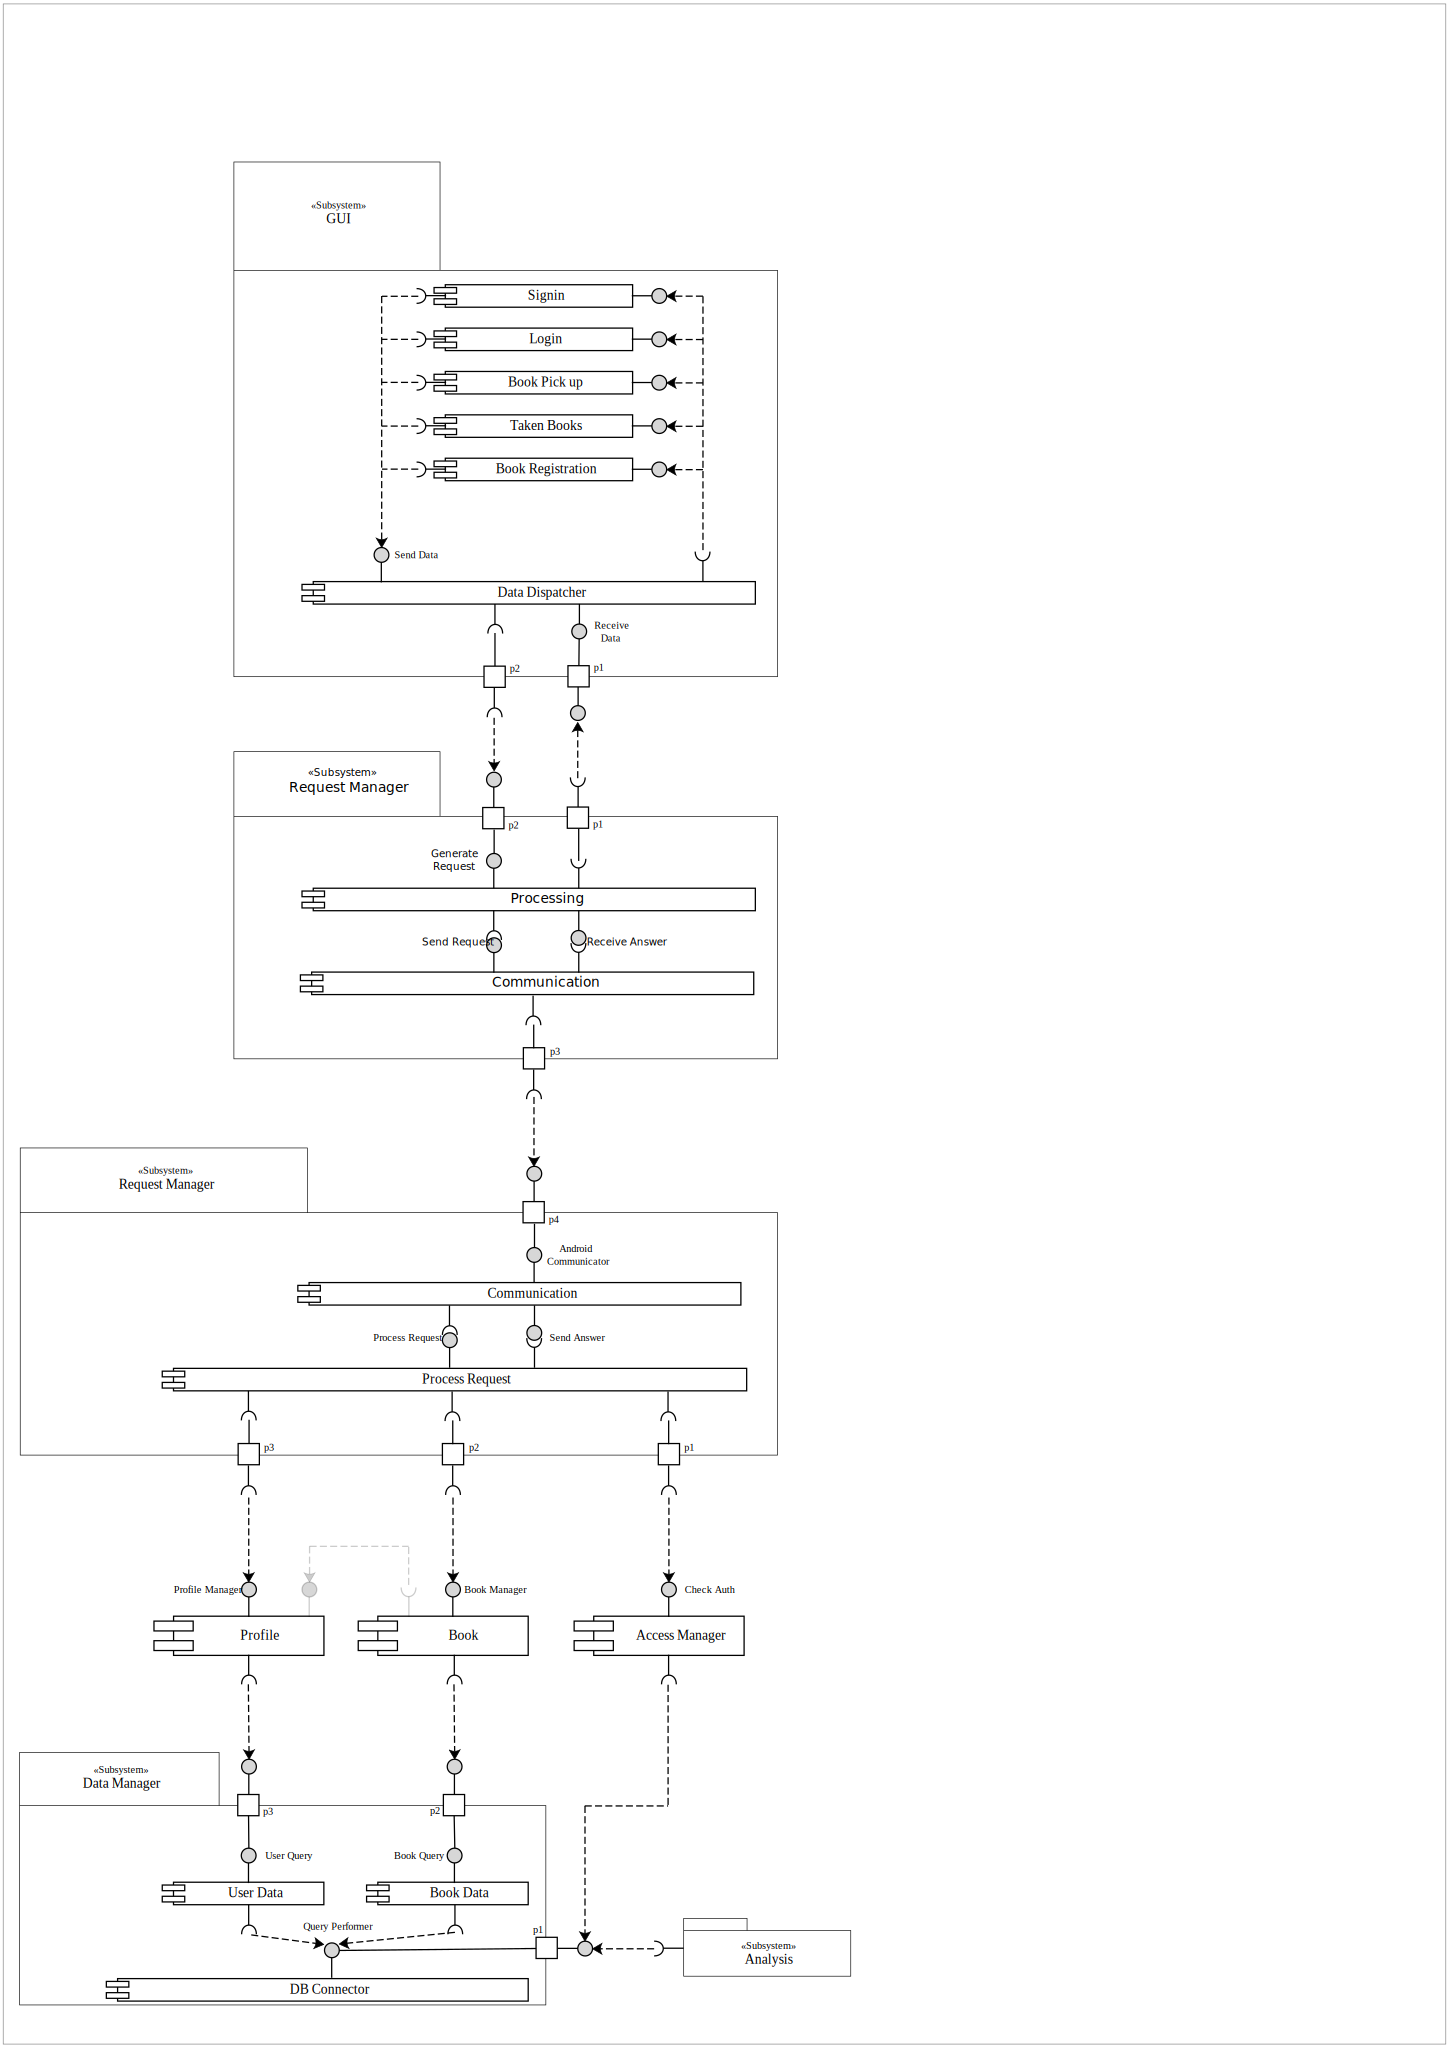
\includegraphics[width=\textwidth]{Immagini/Logical_View}
	\caption{Logical view}
	\label{fig:LogicalView}
\end{figure}

\section{Parte algoritmica: \textit{reservation handler}}
Le gestione delle prenotazioni dei libri è una delle parte innovative introdotte dalla start up: questo servizio mira a sfruttare la flessibilità della community di sharing, basata sull'ideale di open-source, per comunque offrire un seervizio mirato ed attento alle necessità del lettore.
Ogni utente, purchè sia registrato all'interno del servizio di Book-sharing, può prenotare un determinato libro che si trova nello stato "Under reading".

Andiamo ad evidenziare gli attori coinvolti in questa operazione:
\begin{itemize}
	\item \textbf{\underline{Lettore} [L]:} esso rappresenta l'utente, registrato nella community, che possiede il libro oggetto della prenotazione. Indichiamo con:
	\begin{itemize}
		\item \textbf{{\LARGE $r_{L}$}:} raggio d'azione del lettore;
		\item \textbf{{\LARGE $ z_{0} $}:} zona di residenza (espressa come coordinate puntuali).
	\end{itemize}
	\item \textbf{\underline{Prenotanti} [$ P_{i}$ con $i=1,...,N $]:} rappresentano l'insieme degli utenti, tutti interessati ad uno specifico libro in possesso dell'utente \textbf{L}.
	Nello specifico l'indice \textit{i-esimo} indica l'ordine temporale con cui sono giunte le prenotazioni per lo specifico libro.
	Oltre a questa informazione, ogni utente, rappresentando un generico utente della community, avrà fornito, al momento della registrazione, le seguenti informazioni:
	\begin{itemize}
		\item \textbf{{\LARGE $r^{i}_{P}$} con $i=1,...,N $:} raggio d'azione del lettore;
		\item \textbf{{\LARGE $z^{i}_{P}$} con $i=1,...,N $:} zona di residenza.
	\end{itemize}

	L'algoritmo può essere scomposto in due macro-blocchi:
	\begin{itemize}
		\item \textbf{Step 0:} questo fase viene realizzata nel momento in cui il sistema inizia ad analizzare tutti gli utenti che hanno effettuato una prenotazione per un determinato libro che si trova nello stato di "Under reading".
		Tutti gli N prenotanti \textit{$ P_{i} $} vengono ordinati in base alla distanza dal lettore \textit{L}, indipendentemente da quello che è l'ordine temporale con cui è stata effettuata la prenotazione: la quantità di cui si terrà conto sarà quindi
		{\LARGE \begin{equation}
			|z^{p}_{i}-z_{0}|
		\end{equation}}
		Questo ordinamento corrisponde quindi sostanzialmente a creare una \textit{priority queue} in cui si va ad assegnare una maggiore priorità all'utente la cui zona di residenza è più vicina a quella del lettore in possesso del libro.
		\item \textbf{Step 1:} in questo macro-blocco andiamo effettivamente ad applicare l'algoritmo \textit{smart} per poter soddisfare, nella maniera migliore, le esigenze di ogni utente della community.
		
		
		
		
		 
	\end{itemize}
\end{itemize}
\end{document}
